    \documentclass[a4paper,12pt]{article}
    \usepackage{subfig}
    \usepackage{todonotes}
    \begin{document}
\begin{figure}[htbp] %  figure placement: here, top, bottom, or page
   \centering%
   \subfloat[Twenty points for which we are trying to find the convex hull]{%
   \missingfigure[figwidth=0.4\textwidth]{Test}%
%   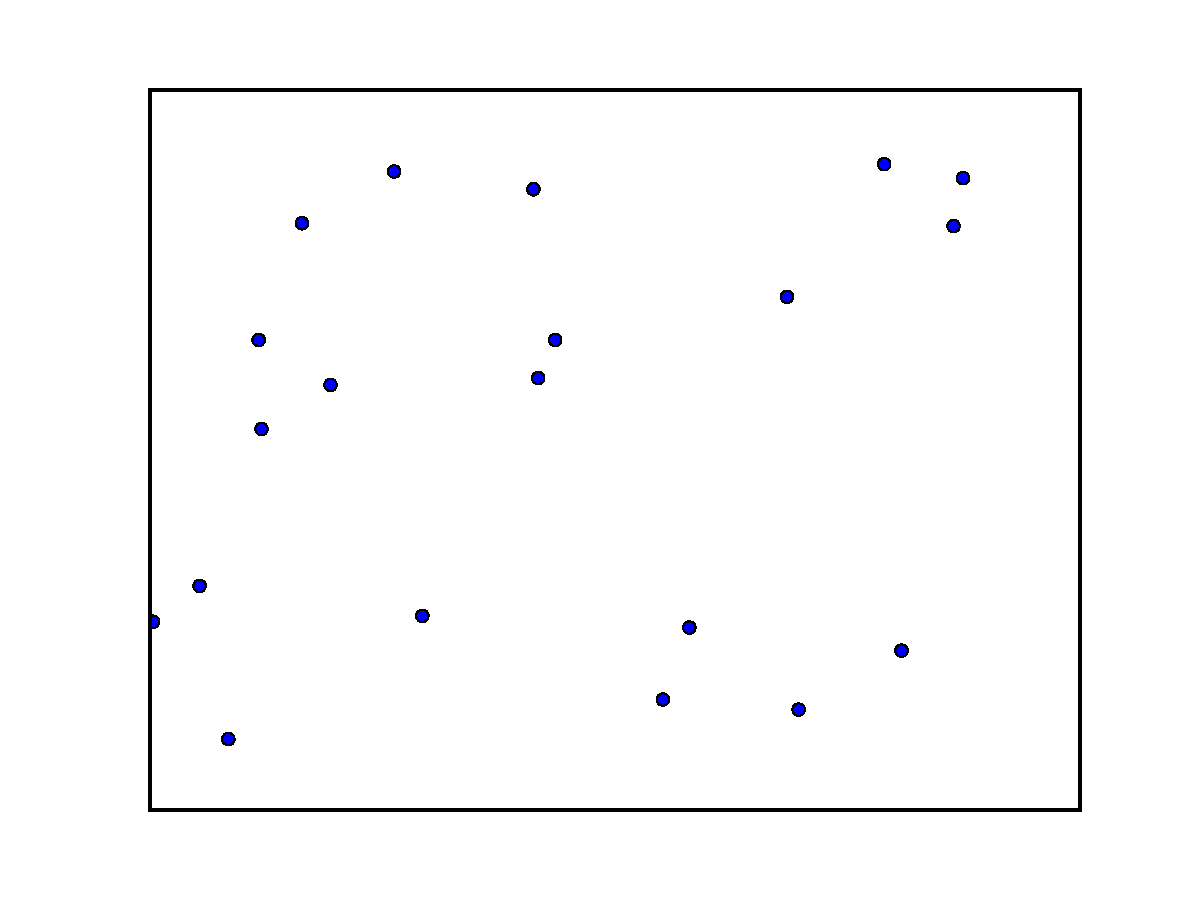
\includegraphics[width=0.4\textwidth]{chapter_ndinterp/plots/qhull_1.pdf}%
   \label{fig:qhull_1}%
 }\quad%
 \subfloat[We find the points with the lowest and highest x-value and connect them with a line]{
   \missingfigure[figwidth=0.4\textwidth]{Test}%
 %  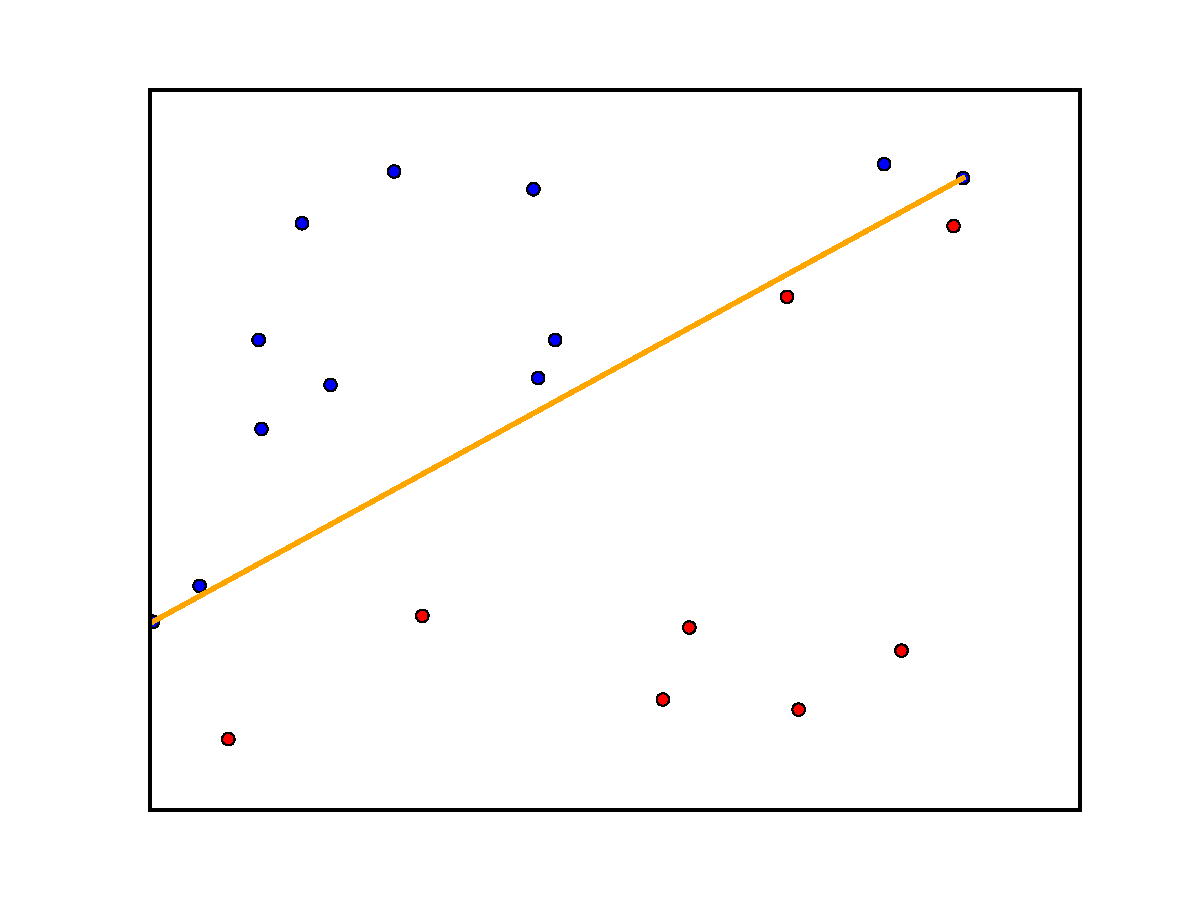
\includegraphics[width=0.4\textwidth]{chapter_ndinterp/plots/qhull_2.pdf}%
   \label{fig:qhull_2}%
 }\\%
 \subfloat[Continuing with the points on the left (same process happens recursively on the right) we find the point furthest away from the line. We then draw two more lines and build a triangle. The points inside of the triangle are not part of the convex hull and are discarded. We will repeat the current step with the two new lines of the triangle. ]{%
   \missingfigure[figwidth=0.4\textwidth]{Test}%
 %  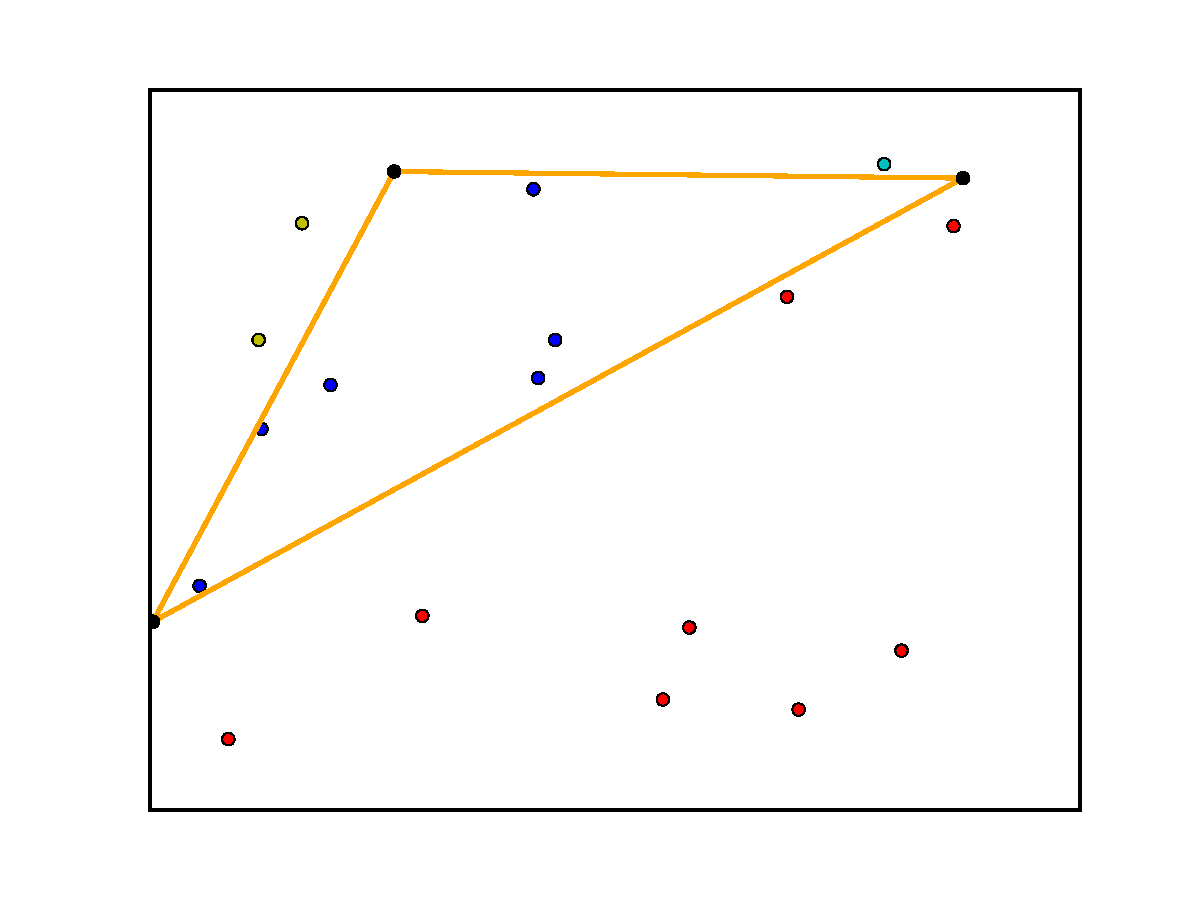
\includegraphics[width=0.4\textwidth]{chapter_ndinterp/plots/qhull_3.pdf}%
   \label{fig:qhull_3}%
 }\qquad%
 \subfloat[We have found points of the convex hull once we can't build a new triangle anymore.]{%
   \missingfigure[figwidth=0.4\textwidth]{Test}%
 %  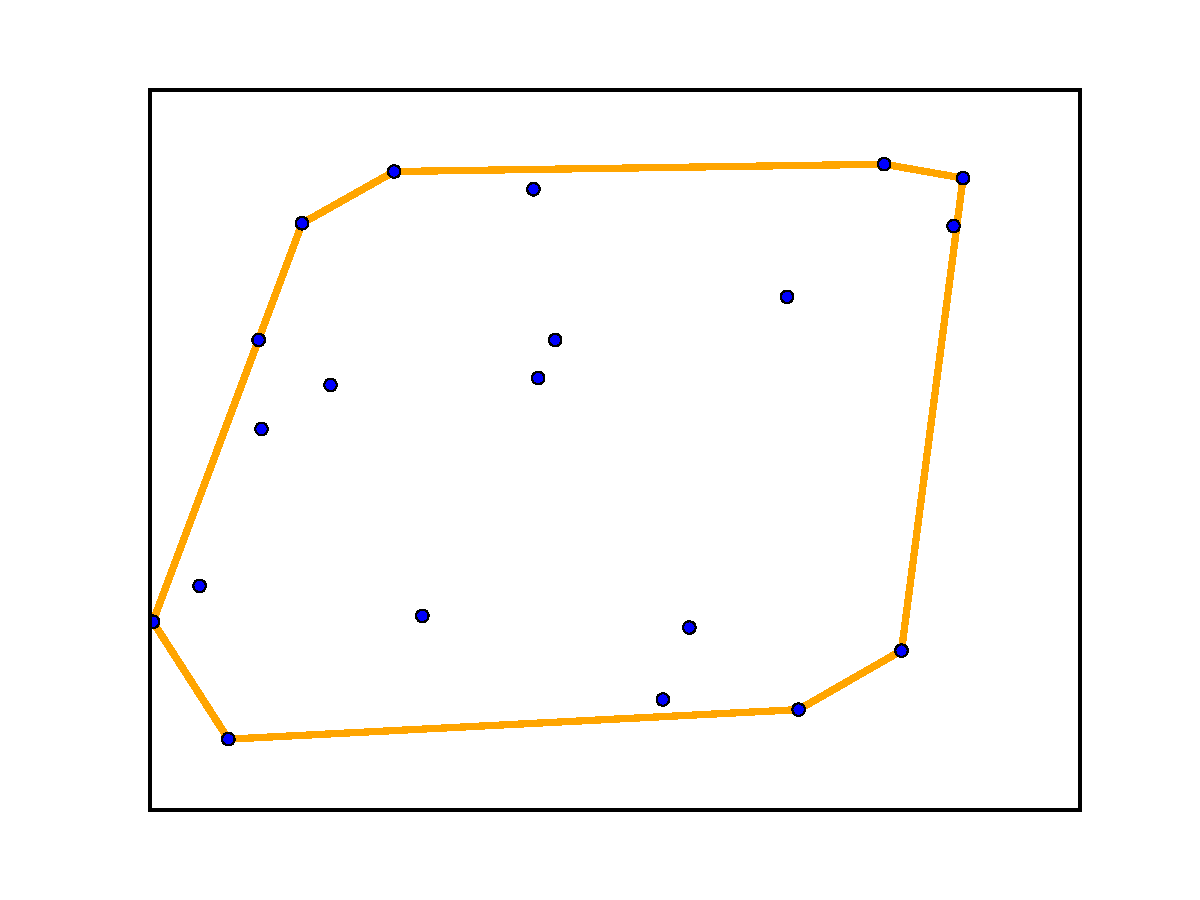
\includegraphics[width=0.4\textwidth]{chapter_ndinterp/plots/qhull_final.pdf}%
   \label{fig:qhull_4}%
 }\quad%
   \caption{Building of a convex hull. }%
   \label{fig:example}%
\end{figure}%
    \end{document}
